% Parlar sobre les modificacions a la placa per adaptar el debugger
% Parlar sobre passar instancies de una classe a la ISR
    % Parlar sobre el problema, la solució utlitizada, perqué aquesta solució (és important que la implementació sigui transparent per l'usuari) i el merge request que va ser denegat per la incompatibilitat amb les plaques (AVR) i que aixo ha comportat fer servir el nostre fork de RadioLib
% Parlar sobre problemes misteriosos
    % Parlar sobre rebre paquets fantasma quan es transmet un paquet (Posar extracte de codi de RadioLib)
    % Parlar sobre diversos crashes en el sistema per culpa de les prioritats i rutines blocants (wdt)
Unfortunately, the development of the research was faced with several issues that ultimately made that fulfilling the original objective of evaluating the performance of a fully functional mesh networking library was impossible. The issues range from using what turned out to be bad sources of information, to ESP32 not being fully compatible with OOP. The following tries to explain in detail what went wrong:
\subsection{TTGO is not compatible with JTAG debuggers}
According to information available at the PlatformIO documentation, the board we use, the TTGO, is completely compatible with any JTAG debugger on the market. However, after ordering the most popular one on the market, we realized that while the debugger needs to be connected to the board through 4 data pins, only 3 of them were exposed to the user, as the fourth was used for the GPS communication with the board, as seen in \autoref{fig:SchematicsTTGO}. After some research and a deep dive into the schematics of the board that are fortunately open source and with the help of Maximilian Gerhard, a kind user on the PlatformIO forum, we discovered that while the pin needed to use the debugger wasn't properly exposed, there was one section of the board that could potentially allow for soldering a regular wire on the desired pin, as shown in \autoref{fig:DebuggerSolutiion}, where the cable should be soldered in the green rectangle.\footnote{The full discussion can be found at \url{https://community.platformio.org/t/ttgo-t-beam-debugging-with-esp-prog/20434}}
\begin{figure}[h!]
    \centering
    \advance\leftskip-4cm
    \advance\rightskip-4cm
    \subfloat[\texttt{IO12} pin transforms into \texttt{RXD1}]{{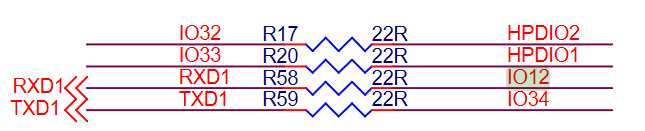
\includegraphics[width=7cm]{Figures/Schematics_1.png}}}%
    \qquad
    \subfloat[\texttt{RXD1} enters the GPS module]{{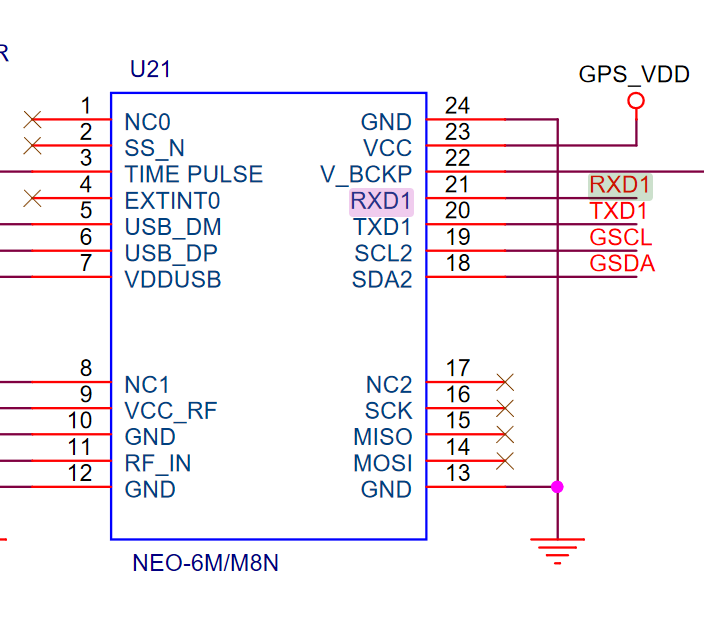
\includegraphics[width=7cm]{Figures/Schematics_2.png}}}%
    \caption[Schematics of the TTGO board]{Schematics of the TTGO board \cite{TTGOSchematics}}%
    \label{fig:SchematicsTTGO}%
\end{figure}

\begin{figure}[h!]
        \centering
        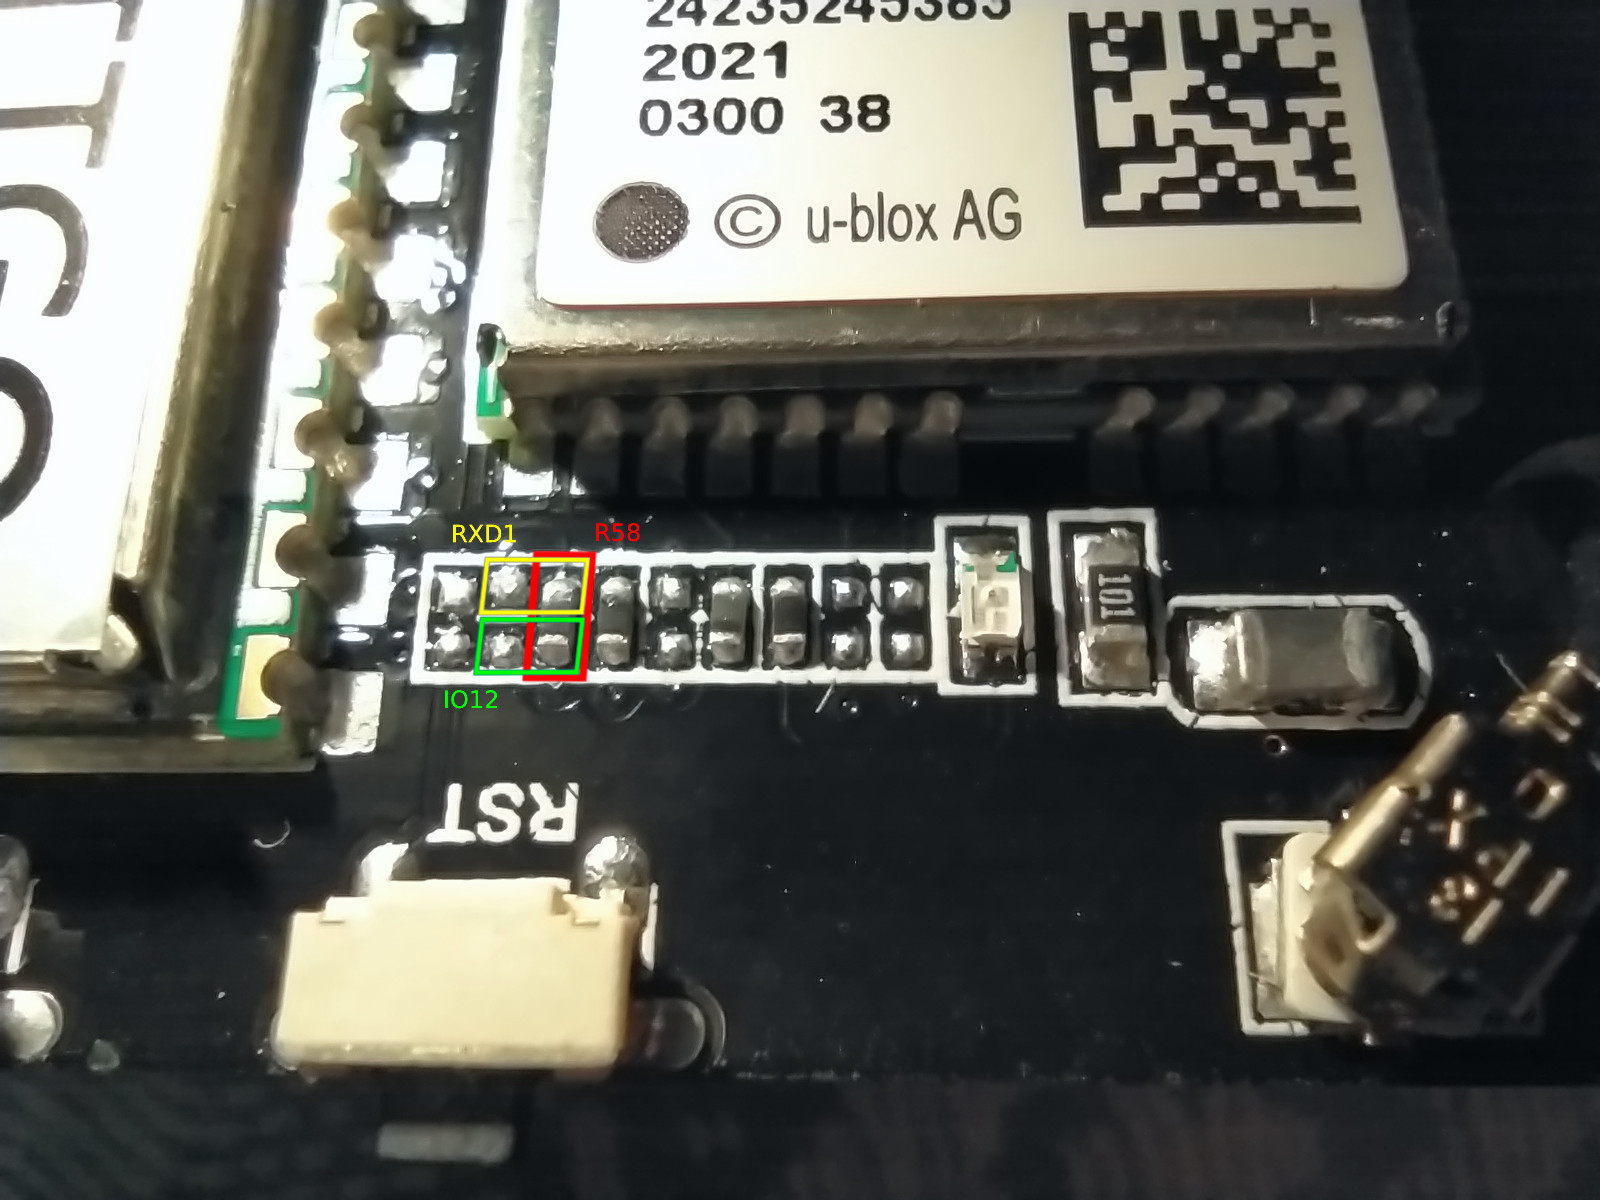
\includegraphics[width=15cm]{Figures/DebuggerSolution.jpeg}
        \caption[TTGO closeup with overlay]{Close up of the TTGO with an overlay indicating what parts of the schematics on \autoref{fig:SchematicsTTGO} are what on the board}
        \label{fig:DebuggerSolutiion}
\end{figure}

\subsection{RadioLib does not fully support OOP}
Even though the choice for RadioLib appeared to be the optimal one at the beginning, as the development progressed, there was one critical issue, the assignation of the ISR didn't support passing member functions, a critical feature if we wanted to develop our code in C++ and have better modularity. The issue was that the RadioLib function that needed to be called in order to set up our custop ISR, \texttt{setDio0Action()} had the signature \texttt{setDio0Action (void(*func)(void))}, but because the function needed to be passed was part of a C++ class, that member function had the signature of \texttt{void MyClass::func(void)}, which does not mach and the compiler refuses to accept. Fortunately, with the use of C++ Standard Library, we made a potential Pull Request for RadioLib that would allow it to accept member functions on the ISR setup call thanks to the \texttt{functional} STD class as seen in \autoref{lst:RadioLibPR}. However, because AVR, which is a supported and very common platform, does not support \texttt{functional}\cite{RadioLibPR}. Thus the pull request was not accepted, but we decided to fork the project and use the version with my slight variation, as it was not expected to use AVR systems for testing and a solution can be thought in the future on how to solve this issue.

\begin{lstlisting}[firstnumber=687, caption={[Fragment of PR]Fragment of the PR that would have allowed RadioLib to accept member functions on ISR setup. The rest of the PR touches some internals of the library. This code section belongs to SX127x.cpp}, label=lst:RadioLibPR,captionpos=b]
void setDio0Action(std::function<void(void)> func);
\end{lstlisting}

\subsection{Receiving data}
In addition to the previous issues with RadioLib, the library also didn't manage  interruption triggering properly as the ISR is called both when receiving data and sending data. This is due to the fact that the interrupt used in RadioLib that triggers it is the same so special attention needs to be put to disable interrupts before sending a message and after sending a message in order to not run the ISR with a nonexistent received message. Unfortunately, the official documentation doesn't mention this part and it caused some confusion while developing as finding the root source of the problem was not trivial.
\subsection{System stability}
The current implementation has some stability issues as it can sometimes crash, usually due to a Watchdog Timer (wdt).
A Watchdog Timer is a mechanism that FreeRTOS uses to make sure the flow of execution is not blocked at some unknown point. The timer needs to be reset periodically and when it is not in a certain amount of time, the system resets as to not lock itself entirely. This issue was introduced when we started using FreeRTOS tasks with higher priority than the main thread. We have been unable to pinpoint the problem but the most likely scenario are the sending and receiving procedures in RadioLib that, for some reason, lock the system and don't allow the WDT to refresh. This has been mitigated by lowering the priority of those tasks.